\subsection{User Study}\label{sec:user}
In this section, we conduct an extensive user study on three real-world applications, i.e., region center identification, reachable route inspection, and traffic flow detection, to demonstrate the superiority of our proposal.
We present our user study setting in Section~\ref{sec:uset}, and analyze the user study results in Section~\ref{sec:uret}.

%To further evaluate the effectiveness of $\avats$ from the the audience perspective, we conducted formal user studies to compare how users perform the urban exploration tasks with visualizations generated by whole dataset, random sampling and $\avats$.


\begin{figure}[t]
	\centering
	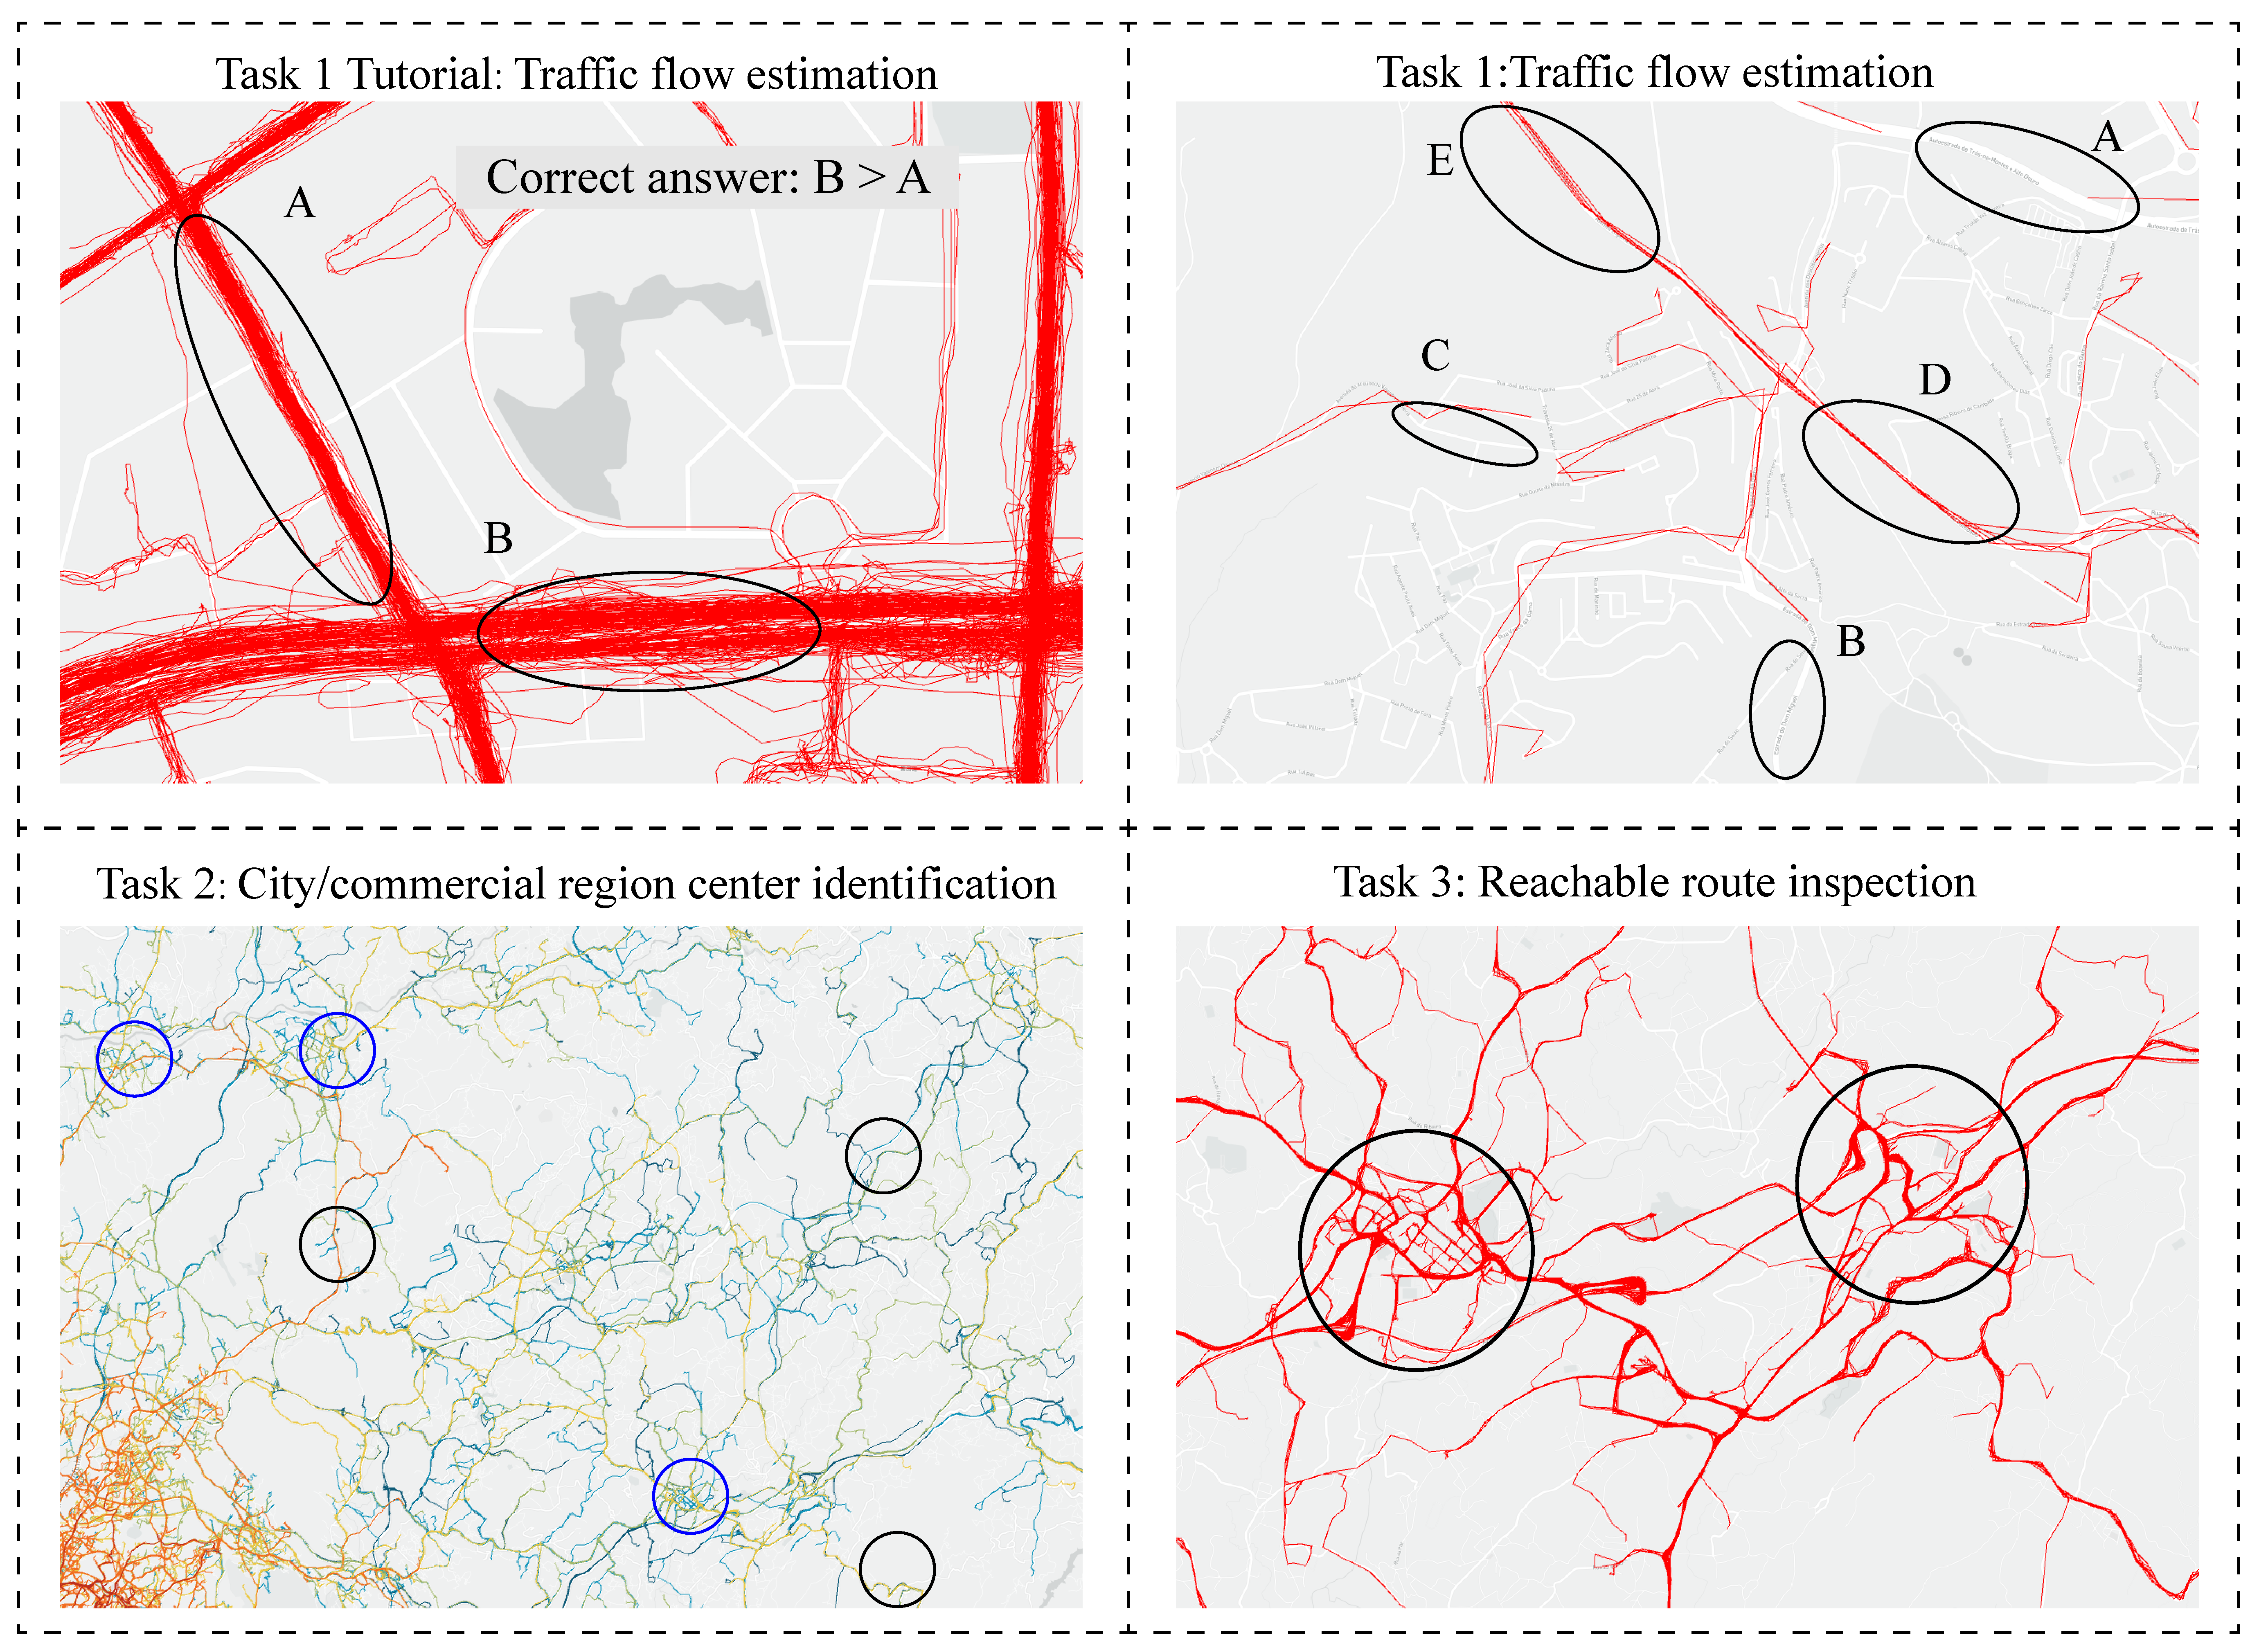
\includegraphics[width=0.44\textwidth]{pictures/user_study/interface.pdf}
	\vspace{-3mm}
	\caption{Three tasks in user study}
	\label{fig:apps}
	\vspace{-6mm}
\end{figure}

\subsubsection{User study setting}\label{sec:uset}

\stitle{Participants and apparatus}
We recruit 186 participants (24 females, 162 males, aged 18 to 29 with mean=21.16, standard derivation =1.48) with normal vision or normal corrected vision.
All participants have the background of computer science.
%, 4.84\% of them have data visualization background.
%The user study system is a web-based platform, which has the size-fixed interface and the participants perform the user study on their own  computers.
%Considering the unfairness caused by different screen sizes, we recommend all participants to set the screen resolution as 1980*1080.
%All images displayed on the interface have the same size 450*300.
The user study system is a web-based platform, all visualized images displayed are with size 450*300.
All participants perform the user study on their own computers.


\stitle{Studied visualization results}
We use the taxi trajectory dataset of \pt{} and \sz{} for the user study.
We study the visualization results which generated by different approaches in three real-world tasks.
We first introduce the studied data generation methods, then elaborate the tasks shortly.

The visualization results we investigated in user study are: (i) full dataset $\full$,
(ii) the result sets of $\rand$ (see Algorithm~\ref{alg:rand}),
(iii) the result sets of $\vats$ with performance optimizations (see Algorithm~\ref{alg:greedy}),
(iv) the result sets of $\avats$ without color encoding,
and (iv) the result sets of $\avats$ with color encoding (see Algorithm~\ref{alg:plus}), denotes as $\cavats$.
The sampling rate is $\alpha = 0.5\%$ and perception tolerance value $\delta = 64$ in all the visualization results in the user study section.
In each task, we use the identical regions with different visualized trajectories, which are returned from the above approaches.


\stitle{User study tasks}
All participants perform three tasks:  (T1) region center identification, (T2) reachable route inspection, and (T3) traffic flow estimation.
%as shown in Fig.~\ref{fig:apps}(A), (B), and (C), respectively.

\sstitle{(T1) region center identification}
The center of the city or commercial region plays an important role in traffic management.
Consequently, the passing taxi trajectories of these centers are more than its surrounding regions, and results in a star-shape cluster of trajectories in the visualization.
In this task, we randomly select 6 different regions which include city or commercial centers from \pt{} and \sz{}.
For each region, we ask the participants to identify the correct city/region center(s) in it.
As shown in Fig.~\ref{fig:apps}(A), it asks the participants to identify 3 correct centers among these 6 cycles by clicking the corresponding cycles.
Specifically, T1 has 30 visualization views in total.
For each region of the visualization views,  we label the locations of the centers in it as the correct centers at first.
We then randomly select other areas which are not centers and far away from the correct centers, and label them as incorrect ones.
The number of correct centers in each visualization view is given to all participates.

%and remove these areas which too close to the correct ones,


% we have generated 145 visualizations(35 for T1, 75 for T2, 35 for T3) and 185 different questions(152 for T1, 21 for T2, 12 for T3).

\sstitle{(T2) reachable route inspection}
Intuitively, the visualized trajectories indicate the reachable routes of different regions.
In this task, we give a visualization view with two circular areas, as illustrated in Fig.~\ref{fig:apps}(B),
then ask the participates to inspect the representative reachable routes between these two areas.
We assume the more trajectories in that route, the more representative it is.
For each visualization view, the number of reachable routes is given.
In T2, we randomly select 7 visualizations of 7 different regions which include two or more cities/commercial districts.
In each region, we choose the identical two circular areas randomly for its \UC{5 different visualization results}.
%, which visualized the returned trajectory set of different approaches.


\sstitle{(T3) traffic flow comparison}
In practice, a road with large traffic flow has many passing trajectories, thus results in a denser and broader trajectory brunch in the visualization.
In the trajectory visualization with color encoding, such kind of pattern can also be highlighted by a concentration of trajectories with \QM{dark} color.
%It is important to preserve the traffic flow information during large trajectory visualization.
In this task, we ask the participates to compare the traffic flows in two roads by the given visualization results, as shown in Fig.~\ref{fig:apps}(C).
In particular, the participants are asked to choose the road with larger traffic flow by clicking the radio box.
They also can choose ``I am not sure'' if they cannot decide the answer.
T3 includes 5 randomly selected regions and each of them has clear road structure.
It has 25 visualization views and 60 road pair comparison in total.
We count the number of passing through trajectories in each road as the exact traffic flow in it.




%\textbf{T1. City/commercial region center identification.}
%% what participants do
%As shown by Fig.~\ref{fig:user_study}(C), a visualization view was given and several regions were marked by circle. The participants needed to select the regions which could be city/commercial centers by click the corresponding circles. In each task, the number of correct regions were given.
%%Why possible
%The city or commercial region centers always have more passing trajectories from different directions than the surrounding regions, which results in the \UC{start-shape} cluster of trajectories in the visualization.
%%Generate the data
%To generate the test data of T1, we randomly chose several visualization views which contain city/commercial regions and labeled the locations of each city/commercial region center on the visualization as the correct locations first.  Then we randomly generated locations and remove the locations close to the correct locations, the remaining locations are the error locations. In each task of T1, with a given visualization, the same number of correct and wrong locations will be randomly selected.
%
%\textbf{T2. Reachable route inspection.}
%% what participants do
%Figure~\ref{fig:user_study}(D) shows the interface of T2, which includes a visualization and two circular regions. The users needed to draw several most representative reachable routes to connect the two regions. The number of the reachable routes is given.
%%Why possible
%The reachable routes indicate the routes connecting two regions, these routes must have the passing trajectories.
%%Generate the data
%To generate the test data, we randomly chose the visualization views which contain two or more city/commercial regions. In each task of T2, a visualization and two regions were randomly selected.

%\textbf{T3. Traffic flow estimation}.
%% what participants do
%As shown by Figure~\ref{fig:user_study}(B), with a given visualization, some road segments will be identified by ellipses(shown as~\ref{fig:user_study}(B)). Several road segment pairs were randomly selected and listed below the view. The participants were asked to choose the one with larger traffic flow by clicking the radio box. They can also choose ``I am not sure'' if they cannot decided the answer.
%%Why possible
%
%%Generate the data
%To generate the test data of T3,  we sampled and selected the visualization views which contain clear road structures. Then the number of trajectories passing through each road segment was counted as the traffic flow.



\stitle{User study procedure}
In the user study system, we first provide a brief introduction about the motivation, tasks and visual encoding scheme, then followed by three tasks.
In each task, we include a tutorial (with correct result) to help the participants familiarizing themselves with the interface, interaction and tasks.
For example, Fig.~\ref{fig:apps}(D) shows a tutorial of T3 in Fig.~\ref{fig:apps}(C), where the traffic flow in road A is smaller than it in road B, as the correct answer shown.
We then randomly choose different views with different questions in each task for different participates.
After they completed all the questions, their answers are collected and saved in the database for the result analysis.
At last, a post-interview was conducted to collect the feedback of the participants.
To evaluate the answers given by the participants, we refer the reviewers to our supplementary video for details of our user study procedure.

%The user study began with the introduction which introduces the motivation, tasks and visual encoding.
%Then the following sessions are divided into three blocks according to the task types. Each block starts with a task tutorial, in which the participants could perform several demo tasks, thus familiarizing themselves with the interface, interaction and tasks. For example, Figure~\ref{fig:user_study}(A) shows the demo task of T3, in which the users can check the correct answer after clicking the ``check'' button. After all the questions are finished, the answers and time usage are collected and saved in the database for the further analysis.

\subsubsection{User study result analysis}\label{sec:uret}
%\TB{Figure~\ref{fig:accuracy} depicts the average accuracy of the different visualization approaches on different tasks from all user study participates.
%Given a task with specified approach, we visualize the average accuracy of all questions by a colored circle and a line-segment to indicate the highest and lowest score of all questions of this task.}
Figure~\ref{fig:accuracy} depicts the average accuracy of all five approaches applied in the three specified tasks.


%\begin{figure}[t]
%	\centering
%	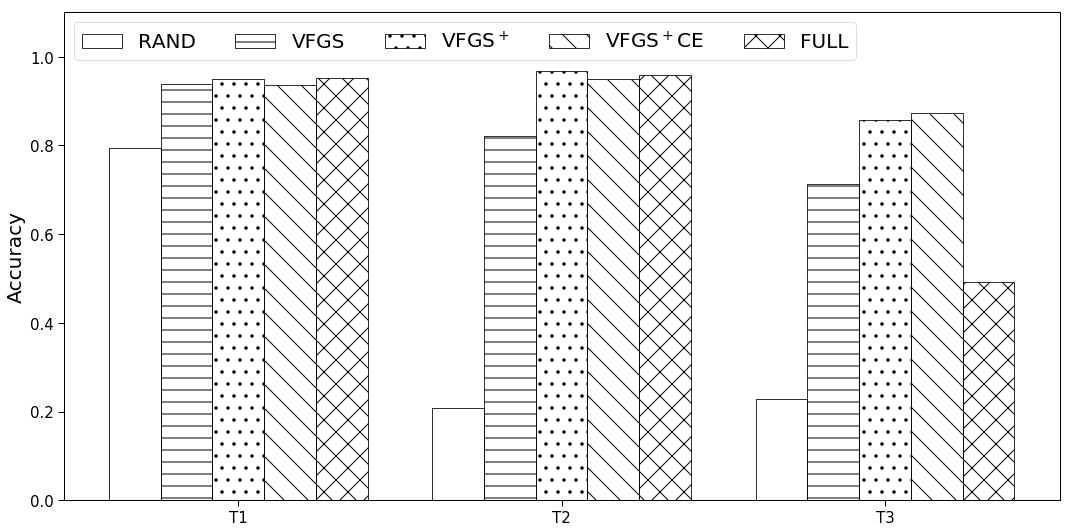
\includegraphics[width=0.40\textwidth]{pictures/user_study/accuracy.png}
%	\vspace{-4mm}
%	\caption{Average accuracy of three types of tasks. X axis indicates the task types. Y axis indicates the accuracy of different approaches.}
%	\label{fig:accuracy}
%	\vspace{-6mm}
%\end{figure}

\begin{figure}[t]
	\centering
	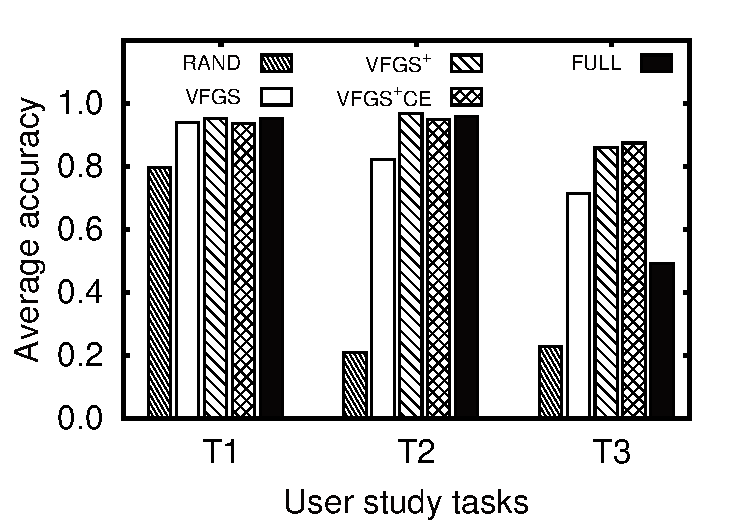
\includegraphics[width=0.3\textwidth]{pictures/userstudy}
	\vspace{-4mm}
	\caption{Average accuracy of three user studied tasks. X axis shows three tasks. Y axis indicates the accuracy of different approaches.}
	\label{fig:accuracy}
	\vspace{-6mm}
\end{figure}

For (T1) region center identification, the average accuracy of our proposed approaches (i.e., $\vats$, $\avats$, and $\cavats$) is higher than its of $\rand{}$ algorithm.
Moreover, our proposed approaches have a very close similar performance with visualizing the full dataset $\full$.
It means the visualized returning results of our proposed approaches worked as excellent as the full data visualization for the exploration of human activity center application.
We observed that the performance of $\cavats$ is slightly worse than performances of $\avats$ and $\full$.
In the post-interview, some of the participants say that the color of trajectories may distract user's attentions and make the cluster characteristics not obvious.


%the participants using all the three proposed methods had a very close performance with the participants using whole dataset, indicating the proposed methods can replace the whole dataset with a guaranteed performance in the exploration of human activity center with trajectory visualization.

For the reachable route inspection study in T2, it is no doubt the $\rand$ has the worst performance among these 5 visualization approaches as it lost many (if not all) detail information.
Unlike center identification, the reachable route inspection are always performed at a fine-grained level of visualization,
which requires good preservation of the detail information, especially, for the sparse regions with few trajectories.
Thus, the advantages of our advanced approaches $\avats$ and $\cavats$ over $\vats$ become obvious and clear.
It owes to our advance approaches taken the data distribution and perception tolerance into consideration explicitly.
%It also is worth to point out our $\avats$ (with average accuracy 0.968) outperforms the visualizations of $\full$ (with average accuracy 0.959) slightly.

%Interestingly,
%For the tasks of T2, $\avats$, $\avats$ with color encoding and the whole dataset all have similar accuracy scores which are far higher than random sampling.
%Moreover, $\avats$ and $\avats$ with color encoding also outperforms the $\vats$ clearly by taking the perception parameters into consideration.
% This results demonstrate the advantage of $\avats$ on the urban exploration at a detail level.


Visually, the task of traffic flow comparison in T3 are more difficult than T1 and T2, which results in relative lower average accuracy for all approaches.  As expected, $\rand$ is the worst.
Interestingly, the average accuracy of visualization views of $\full$ is lower than our proposed approaches, i.e., $\vats,\avats$ and $\cavats$.
In the post-interview, the participants pointed out that many visualization views of $\full$ dataset had serious visual clutter,
which made it is impossible to compare the traffic flows in the two road segments.
The average accuracy of our proposed $\avats$ shows $\avats$ alleviated the visual clutter problem and preserved the clear structure.
$\cavats$ further highlighted the crowded road segments from the surroundings by color, which resulted it has the highest average accuracy in the task T3.

In summary, the qualitative user study of our proposal demonstrates the effectiveness of $\avats$ for large trajectory visualization by three real-world tasks.
All of our proposals ($\vats$, $\avats$, and $\cavats$) outperform the $\rand$ approach significantly.
In addition, the participates achieved equivalent or higher accuracy score in $\avats$ when comparing with the visualization of full dataset $\full$.


\subsection{Qualitative Evaluation}\label{sec:quality}
In this section, we conduct qualitative evaluation of our proposals on \pt{} and \sz{} trajectory datasets from two aspects: (i) the visual fidelity in different zoom levels,
and (ii) the running time with different sampling rates.

\begin{figure}
 \centering
 \small
 \begin{tabular}{cc}
   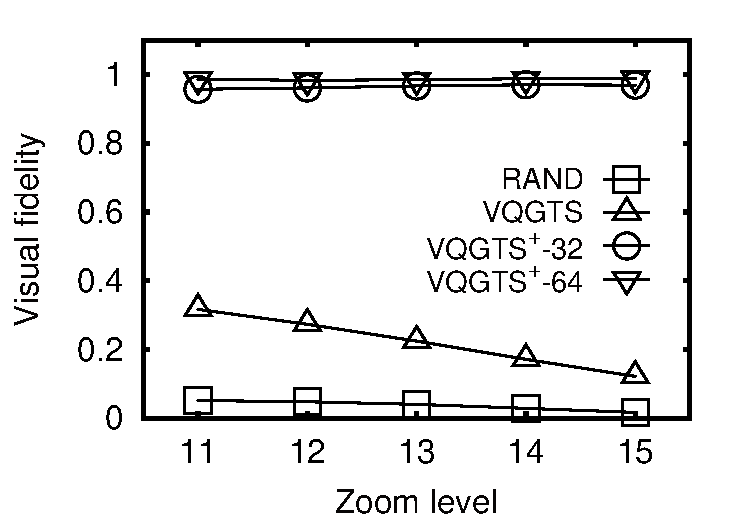
\includegraphics[width=0.44\columnwidth]{fporto}
   &
   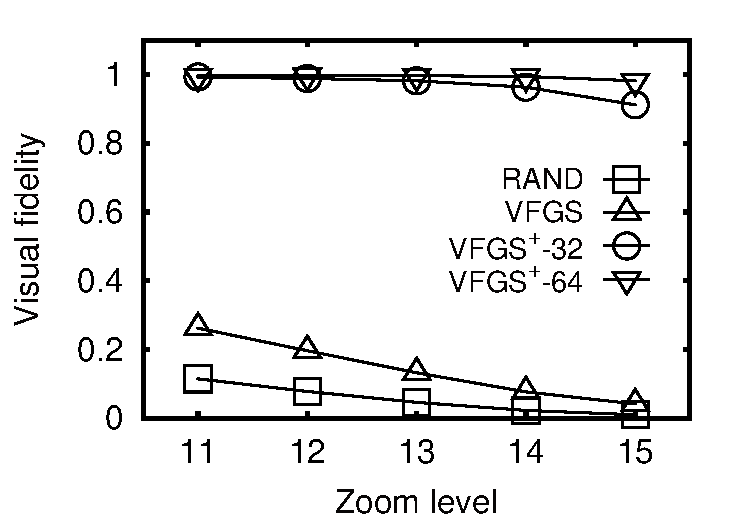
\includegraphics[width=0.44\columnwidth]{fshenzhen}
   \\
   (A) \pt{}
   &
   (B) \sz{}
 \end{tabular}
 \vspace{-2mm}
 \caption{Visual fidelity of proposed approaches}
 \label{fig:fidelity}
 \vspace{-4mm}
\end{figure}

\stitle{Visual fidelity evaluation}
We first evaluate the visual fidelity of our proposed methods.
We measure the visual fidelity of different approaches over the full dataset $\full$ by using the $loss()$ function we defined in Section~\ref{sec:def}.
Fig.~\ref{fig:fidelity} (A) and (B) shows the visual fidelity of $\rand$, $\vats$, $\avats$ with $\delta=32$ and $\avats$ with $\delta=64$ from zoom level 11 to 15(overview to detail view) in
\pt{} and \sz{}, respectively.
We can conclude that: (i) $\rand$ approach did not guarantee the visual fidelity of the result;
(ii) even $\vats$ offers theoretical visual fidelity guarantee w.r.t. the optimal sampled result set with given sampling rate, but it still has room for improving over the $\full$ dataset;
(iii) $\avats$ with $\delta=32$ and $\delta=64$ has excellent visual fidelity w.r.t. the $\full$ dataset. The minimum visual fidelity value is 0.95 and 0.91 in \pt{} and \sz{}, respectively.
It also confirms the superiority of our proposal;
and (iv) the visual fidelity of $\avats$ falls with the rising of zoom levels, e.g., from zoom level 11 to 15.
The reason is the higher zoom level, the more detail information are required.


\begin{figure}
 \centering
 \small
 \begin{tabular}{cc}
   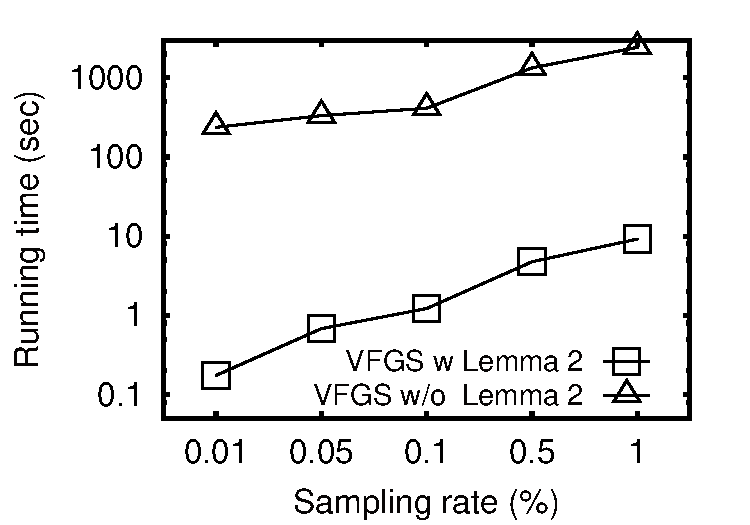
\includegraphics[width=0.44\columnwidth]{tporto}
   &
   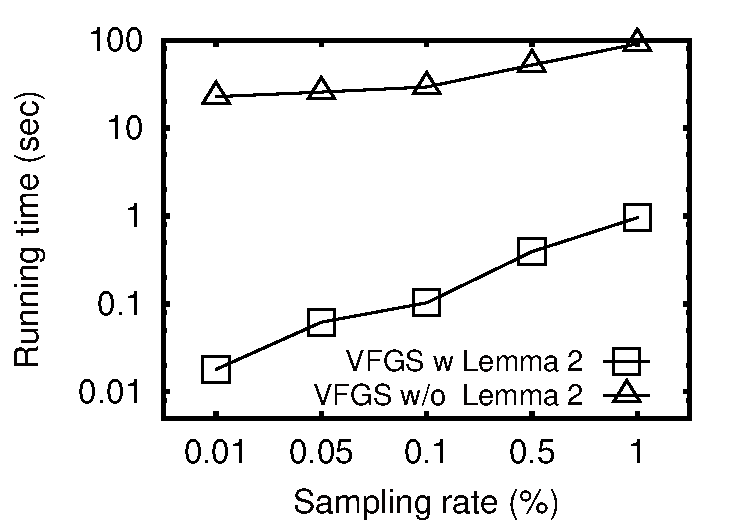
\includegraphics[width=0.44\columnwidth]{tshenzhen}
   \\
   (A) \pt{}
   &
   (B) \sz{}
 \end{tabular}
 \vspace{-2mm}
 \caption{The running time of $\vats$ with or without optimization techniques}
 \label{fig:cost}
 \vspace{-4mm}
\end{figure}


\stitle{Running time evaluation}
Last, we report the running time of our $\vats$ on two datasets: \pt{} and \sz{} by varying the sampling rate from $0.01\%$ to $1\%$.
It is no doubt our visual fidelity guaranteed sampling approach $\vats$ is quite slow without the performance optimizations in Section~\ref{sec:opt}.
Our optimized $\vats$ (e.g., $\vats$ with Lemma~\ref{lem:submodular}) outperform $\vats$ by one to three orders of magnitudes in both \pt{} and \sz{}, as shown in Fig.~\ref{fig:cost}(A) and (B).
Finally, with excellent performance of our $\vats$, we conclude that our proposals support interactive visualization for large trajectory data exploration, i.e., generate visualization results within seconds.

